\documentclass[aspectratio=169]{beamer}

\usepackage[utf8]{inputenc}


\usepackage[pdftex,dvipsnames]{xcolor}  % Coloured text etc.
%\usepackage[top=2cm, bottom=2.5cm, right=2.5cm, left=2.5cm]{geometry} 
%\usepackage{breakurl}
\usepackage{amsmath,amsthm,amssymb,amsfonts,graphicx}
\usepackage{xypic}
\usepackage{stmaryrd}
\usepackage{tikz}
\usetikzlibrary{cd}
\usepackage{proof}
\usepackage[shortlabels]{enumitem}
\usepackage{mathtools}
\usepackage{lscape}
%\usepackage{tocloft}
\usepackage{multicol} 
\usepackage{leftidx}
\usepackage{bbm}
\usepackage{rotating}
\usepackage{extarrows}
\usepackage{graphicx}
\usepackage{placeins}
\usepackage{dsfont}
\usepackage{caption}
%\usepackage{tikz-cd}
%\usepackage[margin=1.4in, top=1in, bottom=1in]{geometry}
%\usepackage{newpxtext}
%\usepackage[varg,bigdelims]{newpxmath}
%\usepackage[backend=biber, backref=true, maxbibnames = 10, style = alphabetic]{biblatex}
%\usepackage[bookmarks=true, colorlinks=true, linkcolor=blue!50!black,
%citecolor=orange!50!black, urlcolor=orange!50!black, pdfencoding=unicode]{hyperref}

\newcommand{\tri
}{\triangleleft
}


\newcommand{\funfact}[1]{\noindent\fbox{\begin{minipage}{\textwidth}
#1
\end{minipage}}}

\newcommand{\s}{{\sf s}}
\renewcommand{\t}{{\sf t}}
\renewcommand{\u}{{\sf{u}}}
\renewcommand{\v}{{\sf{v}}}
\newcommand{\<}{\langle}
\renewcommand{\>}{\rangle}
\newcommand{\X}{\mathbb{X}}
\newcommand{\A}{\mathbb{A}}
\newcommand{\B}{\mathbb{B}}
%\newcommand{\C}{\mathbb{C}}
\newcommand{\D}{\mathbb{D}}
\newcommand{\I}{\mathbb{I}}
\newcommand{\J}{\mathbb{J}}
\newcommand{\N}{\mathbb{N}}
\newcommand{\U}{\mathbb{U}}
\newcommand{\V}{\mathbb{V}}
\newcommand{\Y}{\mathbb{Y}}
\newcommand{\Z}{\mathbb{Z}}
\newcommand{\R}{\mathbb{R}}
\newcommand{\dsa}{$\dag$-$*$-autonomous}  
\newcommand{\dldc}{$\dag$-LDC}  
\newcommand{\m}{{\sf m}}
\newcommand{\f}{{\sf f}}

\newcommand{\Set}{{\sf Set}}
\newcommand{\duo}{\mathsf{duo}}
\newcommand{\indep}{{\sf indep}}
\newcommand{\Cocore}{{\sf Cocore}}
\newcommand{\Poly}{{\sf Poly}}
\newcommand{\lCore}{{\sf core_{\ell}}}
\newcommand{\rCore}{{\sf core_r}}
\newcommand{\nD}{{\sf normalDuo}}
\newcommand{\Iso}{{\sf Isomix}}
\newcommand{\coeval}{{\sf coev}}
\newcommand{\eval}{{\sf ev}}

\newcommand{\dashvv}{\dashv \!\!\!\! \dashv}  
\newcommand{\yon}{\mathcal{y}}
\newcommand{\then}{\fatsemi}

\newcommand{\priyaa}[1]{\textcolor{purple}{#1}}

\newcommand{\nat}{\text{nat. }} 
\newcommand{\id}{{\sf id}} 
\newcommand{\CP}{\mathsf{CP}}
\newcommand{\ox}{\otimes}
\newcommand{\pr}{\oplus}
\newcommand{\oa}{\oplus}
\newcommand{\op}{\mathsf{op}}
\newcommand{\rev}{\mathsf{rev}}
\newcommand{\mx}{\mathsf{mx}}
\newcommand{\Chu}{\mathsf{Chu}}
\newcommand{\FRel}{\mathsf{FRel}}
\newcommand{\FMat}{\mathsf{FMat}}
\newcommand{\Rel}{\mathsf{Rel}}
\newcommand{\Mat}{\mathsf{Mat}}
\newcommand{\Core}{\mathsf{Core}}
\newcommand{\Unitary}{\mathsf{Unitary}}
\newcommand{\dual}{\mathbin{\text{\reflectbox{$\Vdash$}}}}
\newcommand{\fin}{\mathsf{FinSp}}
\newcommand{\lollipop}{\ensuremath{\!-\!\!\circ}}
\renewcommand{\bar}[1]{\overline{#1}}
\newcommand{\x}{\times}
\newcommand {\poppilol} {\reflectbox{$\multimap$}}


%%%%%%%%%%%%%%%%%%%%%%%%%%%%%%%%%%%%%%%%%%%%%%%%%%%%%%%%%%%%%%%%%%%%%%%%%
% M. Barr uses the following:  "It gives a \to that can be used as
% $A\to B$ or $A\to^f B$ or $A\to^{f\o g\o h}B$ or even $A\to^f_gB$.  The
% arrow will grow to fit the label(s).  There are similar definitions for
% \two and \tofro, for which you really might want labels both above and
% below.  Actually, by reading your definition of \kto, I was able to
% simplify this.  But it is still nice to have the optional arguments.
% There is only caveat: although you can have one or the other or both
% labels, if you have both the upper must precede the lower.  These defs
% must either be placed in a style file xor surrounded by \makeatletter
% and \makeatother (but NOT both)."  (Modifications by rags)
% The definitions below look more elaborate than they need to be.
% The reason is that an empty asscript will still cause extra vertical
% spacing and the only way to avoid ugly extra space seems to be using
% some such method as this.

\makeatletter
\newenvironment{myproof}[1][\proofname]{\par
    \pushQED{\qed}%
    \normalfont \topsep6\p@\@plus6\p@\relax
    \trivlist
    \item[\hskip\labelsep
        \itshape
        #1\@addpunct{.} ]\mbox{}\par\nobreak}
    {\popQED\endtrivlist\@endpefalse}
\makeatother

\makeatletter

% In-text size:

\newdimen\w@dth

\def\setw@dth#1#2{\setbox\z@\hbox{\scriptsize $#1$}\w@dth=\wd\z@
\setbox\@ne\hbox{\scriptsize $#2$}\ifnum\w@dth<\wd\@ne \w@dth=\wd\@ne \fi
\advance\w@dth by 1.2em}

\def\t@^#1_#2{\allowbreak\def\n@one{#1}\def\n@two{#2}\mathrel
{\setw@dth{#1}{#2}
\mathop{\hbox to \w@dth{\rightarrowfill}}\limits
\ifx\n@one\empty\else ^{\box\z@}\fi
\ifx\n@two\empty\else _{\box\@ne}\fi}}
\def\t@@^#1{\@ifnextchar_ {\t@^{#1}}{\t@^{#1}_{}}}


\def\t@left^#1_#2{\def\n@one{#1}\def\n@two{#2}\mathrel{\setw@dth{#1}{#2}
\mathop{\hbox to \w@dth{\leftarrowfill}}\limits
\ifx\n@one\empty\else ^{\box\z@}\fi
\ifx\n@two\empty\else _{\box\@ne}\fi}}
\def\t@@left^#1{\@ifnextchar_ {\t@left^{#1}}{\t@left^{#1}_{}}}


\def\two@^#1_#2{\def\n@one{#1}\def\n@two{#2}\mathrel{\setw@dth{#1}{#2}
\mathop{\vcenter{\hbox to \w@dth{\rightarrowfill}\kern-1.7ex
                 \hbox to \w@dth{\rightarrowfill}}%
       }\limits
\ifx\n@one\empty\else ^{\box\z@}\fi
\ifx\n@two\empty\else _{\box\@ne}\fi}}
\def\tw@@^#1{\@ifnextchar_ {\two@^{#1}}{\two@^{#1}_{}}}


\def\tofr@^#1_#2{\def\n@one{#1}\def\n@two{#2}\mathrel{\setw@dth{#1}{#2}
\mathop{\vcenter{\hbox to \w@dth{\rightarrowfill}\kern-1.7ex
                 \hbox to \w@dth{\leftarrowfill}}%
       }\limits
\ifx\n@one\empty\else ^{\box\z@}\fi
\ifx\n@two\empty\else _{\box\@ne}\fi}}
\def\t@fr@^#1{\@ifnextchar_ {\tofr@^{#1}}{\tofr@^{#1}_{}}}

% Displaysize:

\newdimen\W@dth
\def\setW@dth#1#2{\setbox\z@\hbox{$#1$}\W@dth=\wd\z@
\setbox\@ne\hbox{$#2$}\ifnum\W@dth<\wd\@ne \W@dth=\wd\@ne \fi
\advance\W@dth by 1.2em}

\def\T@^#1_#2{\allowbreak\def\N@one{#1}\def\N@two{#2}\mathrel
{\setW@dth{#1}{#2}
\mathop{\hbox to \W@dth{\rightarrowfill}}\limits
\ifx\N@one\empty\else ^{\box\z@}\fi
\ifx\N@two\empty\else _{\box\@ne}\fi}}
\def\T@@^#1{\@ifnextchar_ {\T@^{#1}}{\T@^{#1}_{}}}


\def\T@left^#1_#2{\def\N@one{#1}\def\N@two{#2}\mathrel{\setW@dth{#1}{#2}
\mathop{\hbox to \W@dth{\leftarrowfill}}\limits
\ifx\N@one\empty\else ^{\box\z@}\fi
\ifx\N@two\empty\else _{\box\@ne}\fi}}
\def\T@@left^#1{\@ifnextchar_ {\T@left^{#1}}{\T@left^{#1}_{}}}


\def\Tofr@^#1_#2{\def\N@one{#1}\def\N@two{#2}\mathrel{\setW@dth{#1}{#2}
\mathop{\vcenter{\hbox to \W@dth{\rightarrowfill}\kern-1.7ex
                 \hbox to \W@dth{\leftarrowfill}}%
       }\limits
\ifx\N@one\empty\else ^{\box\z@}\fi
\ifx\N@two\empty\else _{\box\@ne}\fi}}
\def\T@fr@^#1{\@ifnextchar_ {\Tofr@^{#1}}{\Tofr@^{#1}_{}}}


\def\Two@^#1_#2{\def\N@one{#1}\def\N@two{#2}\mathrel{\setW@dth{#1}{#2}
\mathop{\vcenter{\hbox to \W@dth{\rightarrowfill}\kern-1.7ex
                 \hbox to \W@dth{\rightarrowfill}}%
       }\limits
\ifx\N@one\empty\else ^{\box\z@}\fi
\ifx\N@two\empty\else _{\box\@ne}\fi}}
\def\Tw@@^#1{\@ifnextchar_ {\Two@^{#1}}{\Two@^{#1}_{}}}


\def\to{\@ifnextchar^ {\t@@}{\t@@^{}}}
\def\from{\@ifnextchar^ {\t@@left}{\t@@left^{}}}
\def\tofro{\@ifnextchar^ {\t@fr@}{\t@fr@^{}}}
\def\To{\@ifnextchar^ {\T@@}{\T@@^{}}}
\def\From{\@ifnextchar^ {\T@@left}{\T@@left^{}}}
\def\Two{\@ifnextchar^ {\Tw@@}{\Tw@@^{}}}
\def\Tofro{\@ifnextchar^ {\T@fr@}{\T@fr@^{}}}

\makeatother
\newcommand{\vcenteredinclude}[2]{\begingroup
\setbox0=\hbox{\includegraphics[#1]{#2}}%
\parbox{\wd0}{\box0}\endgroup}
% for pullback corner
\newcommand{\pullbackcorner}[1][ul]{\save*!/#1+1.2pc/#1:(1,-1)@^{|-}\restore}
\newcommand{\pushoutcorner}[1][dr]{\save*!/#1-1.2pc/#1:(-1,1)@^{|-}\restore}

%%%%%%%%%%%%%%%%%% TikZ %%%%%%%%%%%%%%%%%%%%%%
\tikzstyle{strings}=[baseline={([yshift=-.5ex]current bounding box.center)}]

%Global tikz scaling

\tikzset{every picture/.append style={scale=.5}, transform shape, strings}

\tikzset{%
symbol/.style={%
draw=none,
every to/.append style={%
edge node={node [sloped, allow upside down, auto=false]{$#1$}}}
}
}

\usetikzlibrary{shapes.geometric}
\usetikzlibrary{patterns}
\usetikzlibrary{fit}
\usetikzlibrary{positioning}
\usetikzlibrary{calc}
\usetikzlibrary{arrows}
\usetikzlibrary{decorations.markings}
\usetikzlibrary{decorations.pathreplacing}
\usetikzlibrary{shapes}

%% -------------------------------------- Declare the layers
\pgfdeclarelayer{nodelayer}
\pgfdeclarelayer{edgelayer}
\pgfsetlayers{edgelayer,nodelayer,main}


%% -------------------------------------- Declare the styles
\tikzset{simple/.style={}}
\tikzset{nothing/.style={outer sep=-3.4pt}}
\tikzset{map/.style={draw,fill=white, rectangle}}
% Edge styles
\tikzstyle{filled}=[-, fill=black]

\tikzset{dot/.style={thick, fill=black, circle, scale=1, inner sep = .05cm}}

\tikzset{oa/.style={draw, scale=0.9,minimum height=.1cm,circle,append after command={
[shorten >=\pgflinewidth, shorten <=\pgflinewidth,]
(\tikzlastnode.north) edge (\tikzlastnode.south)
(\tikzlastnode.east) edge (\tikzlastnode.west)
} } }

\tikzset{ox/.style={draw, scale=0.9,minimum height=.1cm,circle,append after command={
[shorten >=\pgflinewidth, shorten <=\pgflinewidth,]
(\tikzlastnode.north west) edge (\tikzlastnode.south east)
(\tikzlastnode.north east) edge (\tikzlastnode.south west) } } }

\tikzset{circ/.style={
shape=circle, inner sep=1pt, draw}}

% Styles added by Priyaa
\tikzstyle{none}=[inner sep=-1pt]
\tikzstyle{circle}=[shape=circle,draw]

\tikzstyle{onehalfcircle}=[shape=circle, scale=1.5, draw]
\tikzstyle{twocircle}=[shape=circle, scale=2, draw]
\tikzstyle{black}=[shape=circle, fill=black, draw]


\newcommand*{\StrikeThruDistance}{0.15cm}%
\newcommand*{\StrikeThru}{\StrikeThruDistance,\StrikeThruDistance}%

\tikzset{wires/.style={}}

\tikzset{box/.style={inner sep=0pt, thick, draw=black, text height=1.5ex, text depth=.25ex, 
text centered, minimum height=3em, anchor=center}}

%%%%%%%%%%%%%%%%%%%%%%%%%%%%%%%%%%%%%%%%%%%%%%%%%%%%%%%%%%%%%%%%%%%%%%%%

\tikzcdset{every label/.append style = {font = \Large}}

%%%%%%%%%%%%%%%%%%%%%%%%%%%%%%%%%%%%%%%%%%%%%%%%%%%%%%%%%%%%%%%%%%%%%%%%

\newcommand{\linmonw} {\xymatrixcolsep{4mm} \xymatrix{ \ar@{-||}[r]^{\circ} & }}
%\newcommand{\linmonwr} {\xymatrixcolsep{4mm} \xymatrix{ \ar@{-||}[r]^{\triangleright} & }}
\newcommand{\linmonwl} {\xymatrixcolsep{4mm} \xymatrix{ \ar@{-||}[r]^{\otimes\;\tri} & }}
\newcommand{\linmonwr} {\xymatrixcolsep{4mm} \xymatrix{ \ar@{-||}[r]^{\tri\;\otimes} & }}
\newcommand{\linmonwrdavid} {\xymatrixcolsep{4mm} \xymatrix{ \ar@{-||}[r]^{\otimes\;\tri} & }}
\newcommand{\linmonwldavid} {\xymatrixcolsep{4mm} \xymatrix{ \ar@{-||}[r]^{\tri\;\otimes} & }}
\newcommand{\linmondavid} {\xymatrixcolsep{4mm} \xymatrix{ \ar@{-||}[r] & }}

\newcommand{\lincomonb} {\xymatrixcolsep{4mm} \xymatrix{ \ar@{-||}[r]_{\bullet} & }}
\newcommand{\lincomonw} {\xymatrixcolsep{4mm} \xymatrix{ \ar@{-||}[r]_{\circ} & }}
\newcommand{\lincomonwr} {\xymatrixcolsep{4mm} \xymatrix{ \ar@{-||}[r]_{\tri\;\otimes} & }}
\newcommand{\lincomonwl} {\xymatrixcolsep{4mm} \xymatrix{ \ar@{-||}[r]_{\otimes\;\tri} & }}

\newcommand{\linbialgw} {\xymatrixcolsep{4mm} \xymatrix{ \ar@{-||}[r]^{\circ}_{\circ} & }}
\newcommand{\linbialgwl} {\xymatrixcolsep{4mm} \xymatrix{ \ar@{-||}[r]^{\otimes\;\tri}_{\otimes\;\tri} & }}
\newcommand{\linbialgwr} {\xymatrixcolsep{4mm} \xymatrix{ \ar@{-||}[r]^{\tri\;\otimes}_{\tri\;\otimes} & }}
\newcommand{\linbialgwb} {\xymatrixcolsep{4mm} \xymatrix{ \ar@{-||}[r]^{\circ}_{\bullet} & }}


\newcommand{\monoid}[1]{(#1, \mulmap{1.5}{white}: #1 \ox #1 \to #1, \unitmap{1.5}{white}: \yon \to #1)}
\newcommand{\comonoid}[1]{(#1, \comulmap{1.5}{white}: #1 \to #1 \ox #1, \counitmap{1.5}{white}: #1 \to \yon)}
\newcommand{\comonoidb}[1]{(#1, \comulmap{1.5}{black}: #1 \to #1 \ox #1, \counitmap{1.5}{black}: #1 \to \yon)}
\newcommand{\Frob}[1]{(#1, \mulmap{1.5}{white}, \unitmap{1.5}{white}, \comulmap{1.5}{white}, \counitmap{1.5}{white})}
\newcommand{\bFrob}[1]{(#1, \mulmap{1.5}{black}, \unitmap{1.5}{black}, \comulmap{1.5}{black}, \counitmap{1.5}{black})}
\newcommand{\bialg}[1]{(#1, \mulmap{1.5}{white}, \unitmap{1.5}{white}, \comulmap{1.5}{black}, \counitmap{1.5}{black})}
\newcommand{\bialgb}[1]{(#1, \mulmap{1.5}{black}, \unitmap{1.5}{black}, \comulmap{1.5}{white}, \counitmap{1.5}{white})}
\newcommand{\trimonoid}[1]{(#1, \trianglemult{0.65}: #1 \tri #1 \to #1, \triangleunit{0.65}: \yon \to #1)}
\newcommand{\tricomonoid}[1]{(#1, \trianglecomult{0.65}: #1 \to #1 \tri #1, \trianglecounit{0.65}: #1 \to \yon)}


\newcommand{\linbialgwtik} {\begin{tikzpicture}
	\begin{pgfonlayer}{nodelayer}
		\node [style=none] (0) at (-2.8, 1.17) {};
		\node [style=none] (1) at (-1.85, 1.17) {};
		\node [style=none] (2) at (-2, 1.35) {};
		\node [style=none] (3) at (-2, 1) {};
		\node [style=none] (4) at (-1.85, 1) {};
		\node [style=none] (5) at (-1.85, 1.35) {};
		\node [style=none] (6) at (-2.2, 1) {};
		\node [style=none] (7) at (-2.5, 1) {};
		\node [style=none] (8) at (-2.35, 0.82) {};
		\node [style=none] (9) at (-1.6, 1.17) {};
		\node [style=none] (10) at (-3.05, 1.17) {};
		\node [style=circle, scale=0.6] (11) at (-2.35, 1.45) {};
		%\node [style=none] (12) at (-2.25, 0.5) {}; %extra node for spacing
	\end{pgfonlayer}
	\begin{pgfonlayer}{edgelayer}
		\draw (2.center) to (3.center);
		\draw (5.center) to (4.center);
		\draw (0.center) to (1.center);
		\draw (6.center) -- (7.center) -- (8.center) -- (6.center);
	\end{pgfonlayer}
\end{tikzpicture}}


\newcommand{\linmonwtik} {\begin{tikzpicture}
	\begin{pgfonlayer}{nodelayer}
		\node [style=none] (0) at (-2.7, 1.17) {};
		\node [style=none] (1) at (-1.85, 1.17) {};
		\node [style=none] (2) at (-2, 1.35) {};
		\node [style=none] (3) at (-2, 1) {};
		\node [style=none] (4) at (-1.85, 1) {};
		\node [style=none] (5) at (-1.85, 1.35) {};
		\node [style=circle, scale=0.6] (6) at (-2.35, 1.45) {};
		\node [style=none] (7) at (-1.6, 1.17) {};
		\node [style=none] (8) at (-2.95, 1.17) {};
	\end{pgfonlayer}
	\begin{pgfonlayer}{edgelayer}
		\draw (2.center) to (3.center);
		\draw (5.center) to (4.center);
		\draw (0.center) to (1.center);
	\end{pgfonlayer}
\end{tikzpicture}}

\newcommand{\tricomul}[1]{\trianglecomult{#1}}
\newcommand{\trimul}[1]{\trianglemul{#1}}
\newcommand{\tricounit}[1]{\trianglecounit{#1}}
\newcommand{\triunit}[1]{\triangleunit{#1}}

% for multiplication and comultiplication maps
% arguments - scale and color of dot
\newcommand{\mulmap}[2]{
	\begin{tikzpicture}[scale={#1}]
		\begin{pgfonlayer}{nodelayer}
			\node [style=circle, scale=0.4, fill={#2}] (5) at (0.32, 0.25) {};
			\node [style=none] (6) at (0.07, 0.5) {};
			\node [style=none] (7) at (0.57, 0.5) {};
			\node [style=none] (8) at (0.32, 0) {};
			\node [style=none] (9) at (0.64, 0.5) {};
		\end{pgfonlayer}
		\begin{pgfonlayer}{edgelayer}
			\draw [style=none] (8.center) to (5);
			\draw [style=none, bend left, looseness=1.25] (5) to (6.center);
			\draw [style=none, bend right, looseness=1.25] (5) to (7.center);
		\end{pgfonlayer}
	\end{tikzpicture}	
}

% need to specify scale and color of dot
\newcommand{\unitmap}[2]{
\begin{tikzpicture}[scale=#1]
	\begin{pgfonlayer}{nodelayer}
		\node [style=circle, scale=0.4, fill=#2] (0) at (0, 0) {};
		\node [style=none] (1) at (0, -0.4) {};
		\node [style=none] (4) at (0.13, 0) {};
	\end{pgfonlayer}
	\begin{pgfonlayer}{edgelayer}
		\draw [style=none] (0) to (1.center);
	\end{pgfonlayer}
\end{tikzpicture} }

\newcommand{\trianglecomult}[1]{
\begin{tikzpicture}[scale=#1]
	\begin{pgfonlayer}{nodelayer}
		\node [style=none] (0) at (-0.25, 3.75) {};
		\node [style=none] (1) at (-0.5, 3.5) {};
		\node [style=none] (2) at (0, 3.5) {};
		\node [style=none] (3) at (-0.25, 4.25) {};
		\node [style=none] (4) at (0.25, 3) {};
		\node [style=none] (5) at (-0.75, 3) {};
	\end{pgfonlayer}
	\begin{pgfonlayer}{edgelayer}
		\draw [bend left, looseness=1.00] (2.center) to (4.center);
		\draw (0.center) to (1.center);
		\draw (0.center) to (2.center);
		\draw (2.center) to (1.center);
		\draw [in=90, out=-165, looseness=0.75] (1.center) to (5.center);
		\draw (0.center) to (3.center);
	\end{pgfonlayer}
\end{tikzpicture}
}


\newcommand{\trianglecounit}[1]{
\begin{tikzpicture}[scale=#1]
	\begin{pgfonlayer}{nodelayer}
		\node [style=none] (0) at (-0.25, 3.5) {};
		\node [style=none] (1) at (-0.5, 3.25) {};
		\node [style=none] (2) at (0, 3.25) {};
		\node [style=none] (3) at (-0.25, 4.25) {};
		\node [style=none] (4) at (-0.25, 2.8) {};
	\end{pgfonlayer}
	\begin{pgfonlayer}{edgelayer}
		\draw (0.center) to (1.center);
		\draw (0.center) to (2.center);
		\draw (2.center) to (1.center);
		\draw (0.center) to (3.center);
	\end{pgfonlayer}
\end{tikzpicture}~\!\!}

\newcommand{\trianglemult}[1]{
\begin{tikzpicture}[scale=#1]
	\begin{pgfonlayer}{nodelayer}
		\node [style=none] (0) at (-0.25, 3.5) {};
		\node [style=none] (1) at (-0.5, 3.75) {};
		\node [style=none] (2) at (0, 3.75) {};
		\node [style=none] (3) at (-0.25, 3) {};
		\node [style=none] (4) at (0.25, 4.25) {};
		\node [style=none] (5) at (-0.75, 4.25) {};
	\end{pgfonlayer}
	\begin{pgfonlayer}{edgelayer}
		\draw [bend right, looseness=1.00] (2.center) to (4.center);
		\draw (0.center) to (1.center);
		\draw (0.center) to (2.center);
		\draw (2.center) to (1.center);
		\draw [in=-90, out=165, looseness=0.75] (1.center) to (5.center);
		\draw (0.center) to (3.center);
	\end{pgfonlayer}
\end{tikzpicture} }

\newcommand{\triangleunit}[1]{
\begin{tikzpicture}[scale=#1]
	\begin{pgfonlayer}{nodelayer}
		\node [style=none] (0) at (-0.25, 4) {};
		\node [style=none] (1) at (-0.5, 4.25) {};
		\node [style=none] (2) at (0, 4.25) {};
		\node [style=none] (3) at (-0.25, 3.25) {};
		\node [style=none] (4) at (-0.25, 3) {};
	\end{pgfonlayer}
	\begin{pgfonlayer}{edgelayer}
		\draw (0.center) to (1.center);
		\draw (0.center) to (2.center);
		\draw (2.center) to (1.center);
		\draw (0.center) to (3.center);
	\end{pgfonlayer}
\end{tikzpicture}~\!\!}

\newcommand{\comulmap}[2]{
	\begin{tikzpicture}[scale={#1}]
		\begin{pgfonlayer}{nodelayer}
			\node [style=circle, scale=0.4, fill={#2}] (5) at (0.32, 0.25) {};
			\node [style=none] (6) at (0.07, 0) {};
			\node [style=none] (7) at (0.57, 0) {};
			\node [style=none] (8) at (0.32, 0.5) {};
			\node [style=none] (9) at (0.64, 0) {};
		\end{pgfonlayer}
		\begin{pgfonlayer}{edgelayer}
			\draw [style=none] (8.center) to (5);
			\draw [style=none, bend right, looseness=1.25] (5) to (6.center);
			\draw [style=none, bend left, looseness=1.25] (5) to (7.center);
		\end{pgfonlayer}
	\end{tikzpicture}
}

% need to specify scale and color of dot
\newcommand{\counitmap}[2]{
\begin{tikzpicture}[scale=#1, rotate=180]
	\begin{pgfonlayer}{nodelayer}
		\node [style=circle, scale=0.4, fill=#2] (0) at (0, 0) {};
		\node [style=none] (1) at (0, -0.4) {};
		\node [style=none] (4) at (0.13, 0) {};
	\end{pgfonlayer}
	\begin{pgfonlayer}{edgelayer}
		\draw [style=none] (0) to (1.center);
	\end{pgfonlayer}
\end{tikzpicture}
}

\newcommand{\dnote}[1]{{\quad \color{blue}$\lozenge$\;David says:}~#1\;{\color{blue}$\lozenge$}\quad}
\newcommand{\pnote}[1]{{\quad \color{red}$\lozenge$\;Priyaa says:}~#1\;{\color{red}$\lozenge$}\quad}


\newcommand{\biglens}[2]{
     \begin{bmatrix}{\vphantom{f_f^f}#2} \\ {\vphantom{f_f^f}#1} \end{bmatrix}
}
\newcommand{\littlelens}[2]{
     \begin{bsmallmatrix}{\vphantom{f}#2} \\ {\vphantom{f}#1} \end{bsmallmatrix}
}
\newcommand{\coclose}[2]{
  \relax\if@display
     \biglens{#2}{#1}
  \else
     \littlelens{#2}{#1}
  \fi
}


\newcommand{\qqand}{\qquad\textnormal{and}\qquad}

\newcommand{\mygray}[1]{{\color{gray}#1}}

\definecolor{darkMagenta}{HTML}{ff9900}
\definecolor{violet}{HTML}{ff9900}

\usepackage{tabularx}
\usepackage{xcolor,colortbl}
\usepackage{ cmll }
\usepackage{panqueques}

\makeatletter
\def\blfootnote{\gdef\@thefnmark{}\@footnotetext}
\makeatother

\newcommand{\purple}[1]{\textcolor{purple}{#1}} 
\newcommand{\tcolor}[1]{\textcolor{magenta}{#1}}

\title{What kind of linearly distributive categories \\ do polynomial functors form?}
\author{Priyaa Varshinee Srinivasan}
\date{\today}

\begin{document} 

\begin{frame}[noframenumbering,plain]
    \begin{tikzpicture}[remember picture, overlay]
        \fill[black] (current page.south west) rectangle ([xshift=2cm]current page.north west);
    \end{tikzpicture}
    \begingroup  
        %\flushright
        \centering
        {\fontfamily{qag}\selectfont\large\bfseries\color{black}\MyTitle} 
        \par \vspace{1em} \MyAuthor  
        \par \par \vspace{1em} 
\includegraphics[scale=0.5]{pics/Topos.png}
        \par \vspace{-1em} \small{Topos Institute, Berkeley}
        \par \vspace{2em} \small{FMCS 2024, Kananaskis}
        \par \vspace{-0.5em} 
        \small{\MyDate}\par
    \endgroup
\end{frame}

\begin{frame}[noframenumbering, plain]

    \begin{tikzpicture}[remember picture, overlay]
        \fill[black] (current page.south west) rectangle ([xshift=2cm]current page.north west);
    \end{tikzpicture}
    \begingroup  

{\centering
This is joint work with \textcolor{magenta}{David Spivak}. 

\vspace{1em}

\pnote{David's picture}

\vspace{1em}

Our paper is available in \textcolor{magenta}{arXiv: 2407.01849}

}

\endgroup

\end{frame}

\begin{frame}[noframenumbering,plain]

\begin{tikzpicture}[remember picture, overlay]
        \fill[black] (current page.south west) rectangle ([xshift=2cm]current page.north west);
    \end{tikzpicture}
    \begingroup  
        \flushleft
        {\fontfamily{qag}\selectfont\hspace{2 cm}\Large\bfseries\color{black}{Linearly distributive categories}}\vspace{1em}\\
        \hspace{2 cm} Robin Cockett, and Robert Seely. {\em Weakly distributive categories} (1997) \\
    \endgroup
\end{frame}

\iffalse

\begin{frame}{Linear logic}

In 1987, Girard introduced linear logic as a logic for resources manipulation.

\vspace{0.5em}

Classical logic treats statements as truth values; linear logic treats statements as resources which cannot be duplicated or destroyed.

\vspace{-1em}

\begin{align*}
    \textcolor{magenta}{p} &:  \text{to spend a dollar} \\
    \textcolor{magenta}{q} &: \text{to buy an apple} 
\end{align*}

``$p \Rightarrow q$" has the meaning that if a dollar is spent then an apple 
can be bought. 

\vspace{0.5em}

A person can either have \textcolor{magenta}{a dollar} or \textcolor{magenta}{an apple} at a given time but not both. 

\vspace{0.5em}
    
    The word ``linear" refers to this resource sensitivity of the 
    logic.
\end{frame}

\begin{frame}{Categorical semantics of multiplicative linear logic}

{\small
      \begin{table}[h]
        \centering
    	\begin{tabular}{ | l | l | }
        \hline
    	 {\bf Linear logic fragment} & {\bf Connectives}  \\  
       \hline 
       \hline
      Negation & $A^\perp$ \\  
      \hline
    	\cellcolor{red!20}Multiplicative  & \cellcolor{red!20}  $(\ox, 1)$ and $(\parr, \bot)$ \\ 
      \hline
    	Additive & $(\with, \top)$ and $(\oplus, 0)$ \\ 
      \hline
    	Exponentials & $!$ and $?$ \\ 
      \hline
    	\end{tabular}
    \end{table}


}

{\bf Negation}: 

\textcolor{magenta}{p}: to spend a dollar \qquad \qquad 
\textcolor{magenta}{$p^\perp$}: to receive a dollar 

    \vspace{0.25em}

  {\bf Multiplicative fragment}: 

    $(\ox, 1)$: an apple $\ox$ an orange ($p \Rightarrow q \ox r$ means access to resources at the same time; conjunction from classical logic)

    $(\parr, \bot)$ = De Morgan's Rule: $(A^\perp \ox B^\perp)^\perp$ (means don't have access to either resource, so someone else owns it; disjunction from classical logic)

\end{frame}


\begin{frame}{Categorical semantics of multiplicative linear logic}

{\small
      \begin{table}[h]
        \centering
    	\begin{tabular}{ | l | l | }
        \hline
    	 {\bf Linear logic fragment} & {\bf Connectives}  \\  
       \hline 
       \hline
      Negation & $A^\perp$ \\  
      \hline
    	\cellcolor{red!20}Multiplicative  & \cellcolor{red!20}  $(\ox, 1)$ and $(\parr, \bot)$ \\ 
      \hline
    	Additive & $(\with, \top)$ and $(\oplus, 0)$ \\ 
      \hline
    	Exponentials & $!$ and $?$ \\ 
      \hline
    	\end{tabular}
    \end{table}


    \begin{table}[h]
    \centering
	\begin{tabular}{ | l | l | }
    \hline
	 \cellcolor{violet!20}{\bf Linear logic fragment} & \cellcolor{violet!20}{\bf Categorical proof theory}  \\  
   \hline 
   \hline
     \cellcolor{red!20}{MLL} & \cellcolor{red!20}{Linearly distributive categories\footnote{Cockett and Seely (1997) ``Weakly Distributive Categories"} }  \\
   	 \cellcolor{red!20}{ $(\ox, 1)$ and $(\parr, \bot)$ }& \cellcolor{red!20}{$(\X, \ox, \top, \oa, \bot)$}\\
  \hline
	 MLL with negation & $*$-autonomous categories\footnote{Barr (1991) ``$*$-autonomous categories and linear logic"} \\ 
  \hline
    \cellcolor{red!20} Compact MLL &  \cellcolor{red!20} Monoidal categories  \\ 
	 \cellcolor{red!20}($\otimes = \parr$, $1 = \bot$) &  \cellcolor{red!20} $(\X, \ox, I)$  \\
  \hline
	Compact closed categories\footnote{Kelly and Laplaza (1980) ``Coherences for compact closed categories"} & Compact MLL with negation \\ 
  \hline
	\end{tabular}
    \label{Table: MLL} 
\end{table}
}

\end{frame}

\fi

\begin{frame}{Linearly distributive categories}

 {\bf Linearly distributive categories (LDCs)\footnote{Cockett and Seely (1997) ``Weakly distributive categories"}:}
    \[
    (\X, \ox, \top, a_\ox, u_\ox^L, u_\ox^R) ~~~~~~~~~ (\X, \oa, \bot, a_\oa, u_\oa^L, u_\oa^R)
    \]  linked by {linear distributors}: 
    \[\partial^L: A \ox (B \oa C) \rightarrow  (A \ox B) \oa C \]
    \[  \textcolor{gray} {A \times (B + C) \simeq (A \times B) + (A \times C)} \]
    \[ \partial^R: (B \oa C) \ox A \rightarrow  B \oa (C \ox A) \]

    \textbf{Intuition:} At a restaurant the waiter, A, can choose to address either person at the table, B or C. Once assigned to B, A cannot choose C.

    \textit{The distributor is not an equality or isomorphism in general!}
        
    {\bf Monoidal categories:} LDCs in which $\ox = \oa; \top = \bot$ 

    \vspace{1em}
\end{frame}

\begin{frame}{Specturm of LDCs}

        \vspace{0.5em}
    
  \[  \begin{tikzpicture}[scale=2]
        \begin{pgfonlayer}{nodelayer}
            \node [style=circle, scale=2, color=magenta, fill=magenta] (0) at (-5.75, 2.75) {};
            \node [style=circle, scale=2, color=black!80, fill=black!80] (1) at (-3.5, 2.75) {};
            \node [style=circle, scale=2, color=black!60, fill=black!60] (2) at (-1, 2.75) {};
            \node [none, color=white] (99) at (-3.5, 2.75) {?};
            \node [style=circle, scale=2, color=black!40, fill=black!40] (3) at (1.75, 2.75) {};
            \node[style=none, color=white] (99) at (1.75, 2.75) {?};
            \node[style=none, color=white] (99) at (-1, 2.75) {?};
            \node [style=none] (4) at (-7.75, 2.75) {};
            \node [style=circle, scale=2, color=magenta!20, fill=magenta!20] (5) at (4, 2.75) {};
            \node [style=none] (6) at (6, 2.75) {};
            \node [style=none] (7) at (-5.75, 2) {{\large \bf LDC}};
            \node [style=none] (8) at (-3.5, 4.35) {};
            \node [style=none] (9) at (-3.5, 3.85) {};        
            \node [style=none] (10) at (-1, 2) {};
            \node [style=none] (11) at (1.75, 4.1) {};
            \node [style=none] (12) at (1.75, 3.5) {};
            \node [style=none] (13) at (4, 2) {};
            \node [style=none] (14) at (-1, 1.4) {};
            \node [style=none] (15) at (4, 1.5) {};
            \node [style=none] (16) at (-5.75, 1.5) {$(\X, \ox, \top, \oa, \bot)$};
            \node [style=none] (17) at (-3.5, 3.35) { };
            \node [style=none] (13) at (4, 2) {{\bf \large Monoidal} category};
            \node [style=none] (15) at (4, 1.5) {$(\X, \ox, I)$};
        \end{pgfonlayer}
        \begin{pgfonlayer}{edgelayer}
            \draw [dotted] (4.center) to (0);
            \draw (0) to (1);
            \draw (1) to (2);
            \draw (2) to (3);
            \draw (3) to (5);
            \draw [dotted] (5) to (6.center);
        \end{pgfonlayer}
    \end{tikzpicture}\]
    
\end{frame}

\begin{frame}{Mix LDCs}

{\bf Mix category} \footnote{Richard Blute, Robin Cockett, and Robert Seely (2000). "Feedback for linearly distributive categories: traces and fixpoints."}: LDC with $m: \bot \to \top$ called the {\bf mix map} with

\begin{center}
$\indep_{A,B}: A \ox B \to A \oa B :=$
\begin{tikzpicture}
	\begin{pgfonlayer}{nodelayer}
		\node [style=ox] (0) at (0, 0.2500001) {};
		\node [style=circ] (1) at (0.5000001, -0.2500001) {};
		\node [style=circ] (2) at (0, -1) {$\bot$};
		\node [style=map] (3) at (0, -1.75) {m};
		\node [style=circ] (4) at (0, -2.5) {$\top$};
		\node [style=circ] (5) at (-0.5000001, -3.25) {};
		\node [style=oa] (6) at (0, -3.75) {};
		\node [style=nothing] (7) at (0, 0.7499999) {};
		\node [style=nothing] (8) at (0, -4.25) {};
	\end{pgfonlayer}
	\begin{pgfonlayer}{edgelayer}
		\draw (7) to (0);
		\draw (0) to (1);
		\draw [in=45, out=-60, looseness=1.00] (1) to (6);
		\draw [in=120, out=-135, looseness=1.00] (0) to (5);
		\draw (5) to (6);
		\draw (6) to (8);
		\draw [densely dotted, in=-90, out=45, looseness=1.00] (5) to (4);
		\draw (4) to (3);
		\draw (3) to (2);
		\draw [densely dotted, in=-135, out=90, looseness=1.00] (2) to (1);
	\end{pgfonlayer}
\end{tikzpicture}
=
\begin{tikzpicture}
	\begin{pgfonlayer}{nodelayer}
		\node [style=circ] (0) at (-0.5000001, -0.2500001) {};
		\node [style=circ] (1) at (0, -1) {$\bot$};
		\node [style=map] (2) at (0, -1.75) {m};
		\node [style=circ] (3) at (0, -2.5) {$\top$};
		\node [style=circ] (4) at (0.5000001, -3.25) {};
		\node [style=nothing] (5) at (0, 0.7499999) {};
		\node [style=nothing] (6) at (0, -4.25) {};
		\node [style=oa] (7) at (0, -3.75) {};
		\node [style=ox] (8) at (0, 0.2500001) {};
	\end{pgfonlayer}
	\begin{pgfonlayer}{edgelayer}
		\draw [densely dotted, in=-90, out=150, looseness=1.00] (4) to (3);
		\draw (3) to (2);
		\draw (2) to (1);
		\draw [densely dotted, in=-45, out=90, looseness=1.00] (1) to (0);
		\draw (8) to (5);
		\draw (8) to (0);
		\draw [in=135, out=-120, looseness=1.00] (0) to (7);
		\draw (7) to (6);
		\draw (7) to (4);
		\draw [in=-45, out=60, looseness=1.00] (4) to (8);
	\end{pgfonlayer}
\end{tikzpicture} 
\[ (1 \oa (u_\oa^L)^{-1}) (1 \ox (\m \oa 1)) \delta^L(u_\ox^R \oa 1)\]
\end{center}
The \tcolor{indep}\footnote{Also referred to as the mixor} must be natural in $A$ and $B$.

\vspace{0.5em}

\end{frame}

\begin{frame}[noframenumbering]{Mix LDCs (cont...)}

\[
    \begin{tikzpicture}[scale=2]
        \begin{pgfonlayer}{nodelayer}
            \node [style=circle, scale=2, color=magenta, fill=magenta] (0) at (-5.75, 2.75) {};
            \node [style=circle, scale=2, color=magenta!80, fill=magenta!80] (1) at (-3.5, 2.75) {};
            \node [style=circle, scale=2, color=black!60, fill=black!60] (2) at (-1, 2.75) {};
            \node [style=circle, scale=2, color=black!40, fill=black!40] (3) at (1.75, 2.75) {};
            \node [style=none] (4) at (-7.75, 2.75) {};
            \node [style=circle, scale=2, color=magenta!20, fill=magenta!20] (5) at (4, 2.75) {};
            \node [style=none] (6) at (6, 2.75) {};
            \node [style=none] (7) at (-5.75, 2) {{\large \bf LDC}};
            \node [style=none] (8) at (-3.5, 4.35) {{\bf \large Mix} category};
            \node [style=none] (9) at (-3.5, 3.85) {$\m: \bot \to \top$};        
            \node [style=none] (10) at (-1, 2) {};
            \node [style=none] (11) at (1.75, 4.1) {};
            \node [style=none] (12) at (1.75, 3.5) {};
            \node [style=none] (13) at (4, 2) {};
            \node [style=none] (14) at (-1, 1.4) {};
            \node [style=none] (15) at (4, 1.5) {};
            \node [style=none] (16) at (-5.75, 1.5) {$(\X, \ox, \top, \oa, \bot)$};
            \node [style=none] (17) at (-3.5, 3.35) {$\mx: A \ox B \to A \oa B$};
            \node [style=none] (13) at (4, 2) {{\bf \large Monoidal} category};
            \node [style=none] (15) at (4, 1.5) {$(\X, \ox, I)$};
            \node[style=none, color=white] (99) at (1.75, 2.75) {?};
            \node[style=none, color=white] (99) at (-1, 2.75) {?};
        \end{pgfonlayer}
        \begin{pgfonlayer}{edgelayer}
            \draw [dotted] (4.center) to (0);
            \draw (0) to (1);
            \draw (1) to (2);
            \draw (2) to (3);
            \draw (3) to (5);
            \draw [dotted] (5) to (6.center);
        \end{pgfonlayer}
    \end{tikzpicture}
\]
    
\end{frame}

\begin{frame}{Isomix LDCs }

\vspace{0.5em}

    It is an {\bf isomix} category if $m$ is an isomorphism.  

\vspace{1em}

    $m$ being an isomorphism does not make the indep an isomorphism.

\vspace{1em}

    \[ \begin{tikzpicture}[scale=2]
        \begin{pgfonlayer}{nodelayer}
            \node [style=circle, scale=2, color=magenta, fill=magenta] (0) at (-5.75, 2.75) {};
            \node [style=circle, scale=2, color=magenta!80, fill=magenta!80] (1) at (-3.5, 2.75) {};
            \node [style=circle, scale=2, color=magenta!60, fill=magenta!60] (2) at (-1, 2.75) {};
            \node [style=circle, scale=2, color=black!40, fill=black!40] (3) at (1.75, 2.75) {};
            \node [style=none] (4) at (-7.75, 2.75) {};
            \node [style=circle, scale=2, color=magenta!20, fill=magenta!20] (5) at (4, 2.75) {};
            \node [style=none] (6) at (6, 2.75) {};
            \node [style=none] (7) at (-5.75, 2) {{\large \bf LDC}};
            \node [style=none] (8) at (-3.5, 4.35) {{\bf \large Mix} category};
            \node [style=none] (9) at (-3.5, 3.85) {$\m: \bot \to \top$};
            \node [style=none] (10) at (-1, 2) {{\bf \large Isomix} category};
            \node [style=none] (13) at (4, 2) {{\bf \large Monoidal} category};
            \node [style=none] (14) at (-1, 1.4) {$\bot \to^{\m}_{\simeq} \top$};
            %\node [style=none] (15) at (4, 1.5) {$\m = 1$, $\mx=1$};
            \node [style=none] (16) at (-5.75, 1.5) {$(\X, \ox, \top, \oa, \bot)$};
            \node [style=none] (17) at (-3.5, 3.35) {$\mx: A \ox B \to A \oa B$};
            \node [style=none] (15) at (4, 1.5) {$(\X, \ox, I)$};
            \node[style=none, color=white] (99) at (1.75, 2.75) {?};
        \end{pgfonlayer}
        \begin{pgfonlayer}{edgelayer}
            \draw [dotted] (4.center) to (0);
            \draw (0) to (1);
            \draw (1) to (2);
            \draw (2) to (3);
            \draw (3) to (5);
            \draw [dotted] (5) to (6.center);
        \end{pgfonlayer}
    \end{tikzpicture} \]
\end{frame} 


\begin{frame}{Compact LDCs}

A {\bf compact LDC} is an LDC in which every indep is an isomorphism. 
\[ \indep_{A,B}: A \ox B \to^{\simeq}  A \oa B \]

\vspace{1.5em}
 
Compact LDCs $(\X, \ox, \top, \oa, \bot)$ are linearly equivalent to the underlying 
monoidal categories $(\X, \ox, \top)$ and $(\X, \oa, \bot)$.    
\end{frame}

 \begin{frame}{Spectrum of LDCs}

    \[    \begin{tikzpicture}[scale=2]
        \begin{pgfonlayer}{nodelayer}
            \node [style=circle, scale=2, color=magenta, fill=magenta] (0) at (-5.75, 2.75) {};
            \node [style=circle, scale=2, color=magenta!80, fill=magenta!80] (1) at (-3.5, 2.75) {};
            \node [style=circle, scale=2, color=magenta!60, fill=magenta!60] (2) at (-1, 2.75) {};
            \node [style=circle, scale=2, color=magenta!40, fill=magenta!40] (3) at (1.75, 2.75) {};
            \node [style=none] (4) at (-7.75, 2.75) {};
            \node [style=circle, scale=2, color=magenta!20, fill=magenta!20] (5) at (4, 2.75) {};
            \node [style=none] (6) at (6, 2.75) {};
            \node [style=none] (7) at (-5.75, 2) {{\large \bf LDC}};
            \node [style=none] (8) at (-3.5, 4.35) {{\bf \large Mix} category};
            \node [style=none] (9) at (-3.5, 3.85) {$\m: \bot \to \top$};
            \node [style=none] (10) at (-1, 2) {{\bf \large Isomix} category};
            \node [style=none] (11) at (1.75, 4.1) {{\bf \large Compact} LDC};
            \node [style=none] (12) at (1.75, 3.5) {$A \ox B \to^{\mx}_{\simeq} A \oa B$};
            \node [style=none] (13) at (4, 2) {{\bf \large Monoidal} category};
            \node [style=none] (14) at (-1, 1.4) {$\bot \to^{\m}_{\simeq} \top$};
            \node [style=none] (15) at (4, 1.5) {$\m = 1$, $\mx=1$};
            \node [style=none] (16) at (-5.75, 1.5) {$(\X, \ox, \top, \oa, \bot)$};
            \node [style=none] (17) at (-3.5, 3.35) {$\mx: A \ox B \to A \oa B$};
        \end{pgfonlayer}
        \begin{pgfonlayer}{edgelayer}
            \draw [dotted] (4.center) to (0);
            \draw (0) to (1);
            \draw (1) to (2);
            \draw (2) to (3);
            \draw (3) to (5);
            \draw [dotted] (5) to (6.center);
        \end{pgfonlayer}
    \end{tikzpicture} \]
    
\end{frame}

\begin{frame}{Symmetry and $\ox$-symmetry}

A \tcolor{symmetric LDC} is an LDC in which $\ox$ and the $\oa$ products are symmetric and the diagram commutes.
\[ \begin{tikzcd}[ampersand replacement=\&]
(A \oa B) \ox C \ar[d, "\tcolor{\partial^R}"'] \ar[r, "\sigma_\ox" ]
	\& C \ox (A \oa B) \ar[r, "\sigma_\oa"]  
	\& C \ox (B \oa A) \ar[d, "\tcolor{\partial^L}"] \\ 
A \oa (B \ox C) 
	\& A \oa (C \ox B)  \ar[l, "\sigma_\oa"]
	\& A \oa (B \ox C) \ar[l, "\sigma_\ox"] 
\end{tikzcd}\]

\vspace{1em}

A \tcolor{$\ox$-symmetric LDC} is an LDC in which the $\ox$ product is symmetric and the $\oa$ product is non-symmetric.

\end{frame}

\begin{frame}{Typical examples of LDCs}

\vspace{2em}

Every monoidal category is an LDC.

\vspace{0.75em}

A bounded distributive lattice regarded as a category is an LDC.

\vspace{0.75em}

All $*$-autonomous categories are LDCs: \\
Ehrhard’s finiteness spaces, Girard's coherence spaces, Chu spaces.

\vspace{1.5em}

\begin{center} 

\textcolor{purple}{\Large Can we have a simple yet a structurally rich example of LDCs?}

\vspace{0.5em}

{\Large Yes!!}

\end{center}

\end{frame}


\begin{frame}{This talk is about ... }

\vspace{1em}

\textcolor{purple}{Poly} the category of polynomial functors and transformations as an example of LDCs.

\vspace{1em}

We will find non-trivial examples of various {structures of LDCs} in Poly.

\vspace{1em}

We will also {discover new properties} of LDCs by studying Poly.

\vspace{2em}

\begin{center} \textcolor{magenta}{Poly seems to be a golden goose for LDCs!!!} \end{center}
   
\end{frame}

\begin{frame}{Acknowledgement}
    \centering
    
    Thanks to Harrison Grodin and Reed Mullanix for their conjecture, that normal duoidal categories are linear distributive categories, which spawned this work.
    
\end{frame}

\begin{frame}{ Recap: Polynomial functors and natural transformations}

\vspace{1em}

A {\bf polynomial functor} is a functor that is isomorphic to a coproduct of representables

 \[ p \cong \sum_{P : p(1)} y^{p[P]} : {\sf Set \to Set} \] 

\vspace{1em}

A schematic of a polynomial functor map, $\varphi: (y^3 + y^2) \to (y + y^2)$.
\[ 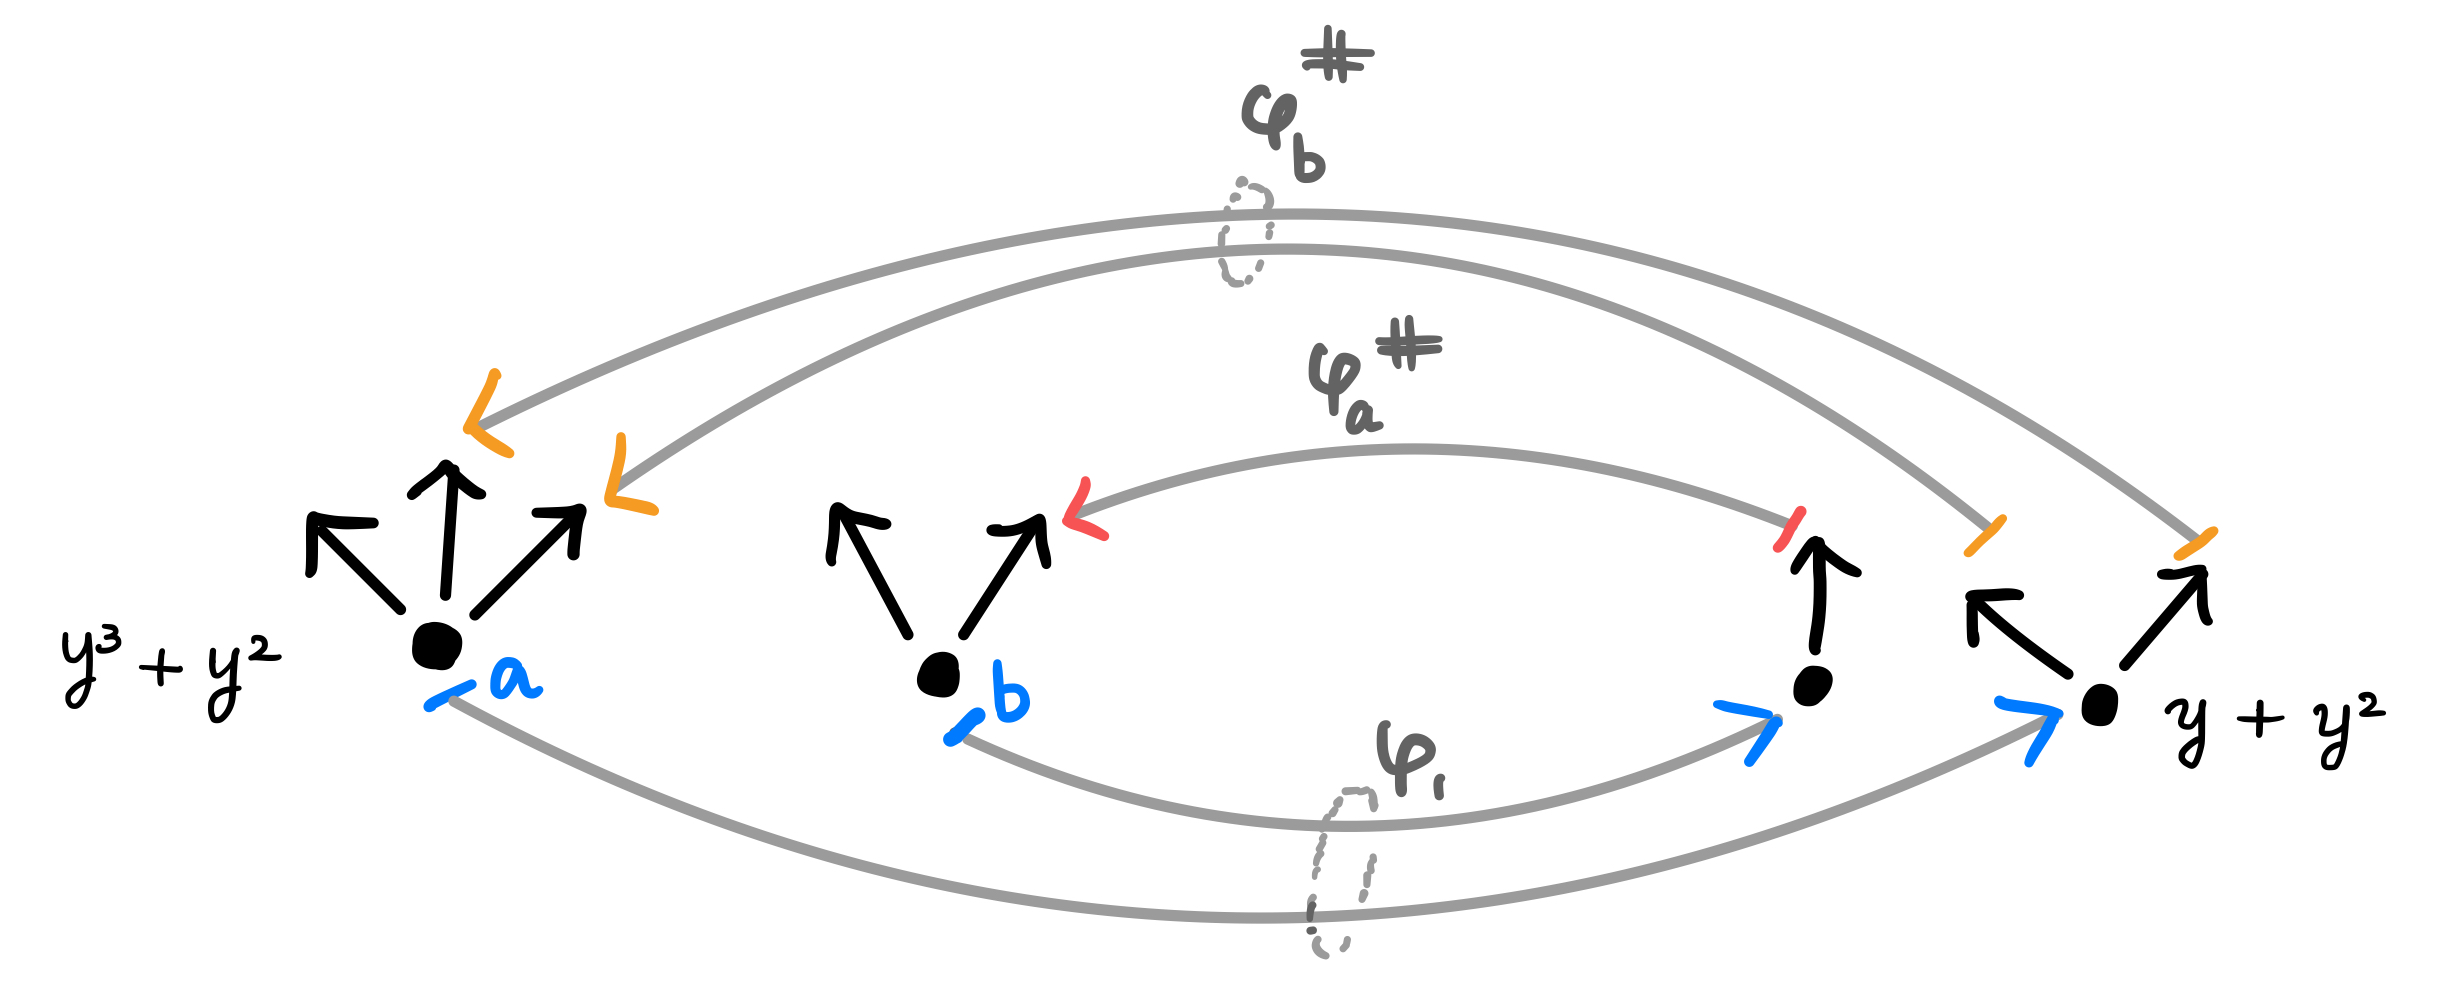
\includegraphics[scale=0.08]{pics/corolla-map.jpeg} \] 
\end{frame}

\begin{frame}{ Recap: Tensor product in Poly}

The tensor product $\ox$ is given by the Day convolution of Cartesian product $\times$ in $\Set$.  

\[ p \ox q = \sum_{P: p(1)} y^{p[P]} \ox \sum_{Q: q(1)} y^{q[Q]} := \sum_{(P,Q): p(1) \times q(1)} y^{p[P] \times q[Q]} \] 

Tensor product $\ox$ is symmetric.

\end{frame}


\begin{frame}{Recap: Tri product in Poly}

The substitution product $\tri$ is given by functor composition. 

\[ p \tri q = \sum_{P: p(1)} y^{p[P]} \tri \sum_{Q: q(1)} y^{q[Q]} :=  
 \sum_{P: p(1)} \Big(\sum_{Q: q(1)} y^{q[Q]} \Big)^{p[P]} 
 = \sum_{P:p(1)} \sum_{\color{purple}{f:p[P] \to q(1)}} \prod_{d:p[P]} \prod_{\color{purple}{e:q[f(d)]}} y \]
 
Read $p \tri q$ as \textcolor{purple}{q then p}.

\vspace{1em}

The tri product $\tri$ is non-symmetric.

\pnote{Add a picture here of composed corolla}

\end{frame}

\begin{frame}[noframenumbering,plain]

\begin{tikzpicture}[remember picture, overlay]
        \fill[black] (current page.south west) rectangle ([xshift=2cm]current page.north west);
    \end{tikzpicture}
    \begingroup  
        \flushleft
        {\fontfamily{qag}\selectfont\hspace{2 cm}\large\color{black}{The category Poly is a $\ox$-symmetric isomix LDC}} \vspace{1em}
         
    \endgroup
\end{frame}

\begin{frame}{Duoidal categories}

   A \tcolor{duoidal category}\footnote{Marcelo Aguiar and Swapneel Arvind Mahajan. Monoidal functors, species and Hopf algebras (2010)} is a category $\X$ with two monoidal structures $(\X, \ox, \top)$ and $(\X, \oa, \bot)$ along with a natural transformation:
    \[ {\duo: ~(a \oa b) \ox (c \oa d) \to (a \ox c) \oa (b \ox d)} \]
    called the \tcolor{interchange law}, and morphisms:
    \[ e_\top: ~\top \to \top \oa \top \quad \quad  e_\bot: ~\bot \otimes \bot \to \bot \]    
    such that the functors $\oa$ and $\bot$ are $\ox$-lax monoidal, and the assosciativity and unitor natural isomorphisms of $(\oa, \bot)$ are $\ox$-monoidal natural transformations.
\vspace{1em}

\end{frame}

\begin{frame}{Normal duoidal category}
 
 In a duoidal category, we have a map $\tcolor{k: \top \to \bot}$

\[ \top \to^{\cong}  \top \ox \top \to^{\cong}  (\top \oa \bot) \ox (\bot \oa \top) \to^{\duo} (\top \ox \bot) \oa (\top \ox \bot) \to^{\cong} \bot \oa \bot \to^{\cong} \bot \] 

\vspace{0.5 em}

A duoidal category is \tcolor{normal} if the above composite is an isomorphism.

\end{frame}

\begin{frame}{Bilax duoidal functors}

Functors...

\end{frame}

\begin{frame}{Normal duoidal is also isomix}

\vspace{1em}

\tcolor{Isomix} category of isomix LDCs and isomix functors

\vspace{1em}

\tcolor{normalDuo} category of normal duoidal categories and bilax duoidal functors

\vspace{1em}

{\bf Theorem:} There is a faithful functor from \tcolor{normalDuo} to \tcolor{Isomix}.

\vspace{1em}

 The category $($Poly$, \otimes, \tri,  y )$ is normal duoidal hence an isomix LDC. Poly is  $\ox$-symmetric.
    
\vspace{1em}

\color{violet}{\bf Attention:} \color{black} Since in this tutorial we will mostly be in a $\ox$-symmetric setting, we will \\ \tcolor{use $\tri$ instead of $\oa$}.    
    
\end{frame}




\begin{frame}[noframenumbering,plain]
\begin{tikzpicture}[remember picture, overlay]
        \fill[black] (current page.south west) rectangle ([xshift=4cm]current page.north west);
    \end{tikzpicture}
    \begingroup  
        \flushleft
        {\fontfamily{qag}\selectfont\hspace{2 cm}\Large\bfseries\color{black}{Meet the linear duals}}\vspace{1em}\\
    \endgroup
\end{frame}

\begin{frame}{What is a linear dual?}
    
    In an LDC, an object $A$ is left dual to $B$ if there exist:
    \[ \eta: \top \to A \tri B ~~~~~~~~ \epsilon: B \ox A \to \bot \]
    such that: 
 
     \[	\begin{tikzpicture}[scale=1.2]
    			\begin{pgfonlayer}{nodelayer}
    				\node [style=none] (6) at (1, 0) {};
    				\node [style=none] (7) at (1, 1) {};
    				\node [style=none] (8) at (2, 1) {};
    				\node [style=none] (9) at (2, 0.75) {};
    				\node [style=none] (10) at (3, 0.75) {};
    				\node [style=none] (11) at (3, 2) {};
    				\node [style=none, scale=1.2] (12) at (1.5, 1.75) {$\eta$};
    				\node [style=none, scale=1.2] (13) at (2.5, 0.1) {$\epsilon$};
    				\node [style=none] (14) at (0.75, 0.25) {$A$};
    				\node [style=none] (15) at (3.25, 1.75) {$A$};
    			\end{pgfonlayer}
    			\begin{pgfonlayer}{edgelayer}
    				\draw (6.center) to (7.center);
    				\draw [bend left=90, looseness=1.50] (7.center) to (8.center);
    				\draw (8.center) to (9.center);
    				\draw [bend right=90, looseness=1.50] (9.center) to (10.center);
    				\draw (10.center) to (11.center);
    			\end{pgfonlayer}
    		\end{tikzpicture} = 
            \begin{tikzpicture}[scale=1.2]
    		  \draw (0,2.5) -- (0,0);
    		\end{tikzpicture} ~~~~~~~~~~
    		\begin{tikzpicture}[scale=1.2]
    			\begin{pgfonlayer}{nodelayer}
    				\node [style=none] (6) at (3, 0) {};
    				\node [style=none] (7) at (3, 1) {};
    				\node [style=none] (8) at (2, 1) {};
    				\node [style=none] (9) at (2, 0.75) {};
    				\node [style=none] (10) at (1, 0.75) {};
    				\node [style=none] (11) at (1, 2) {};
    				\node [style=none, scale=1.2] (12) at (2.5, 1.75) {$\eta$};
    				\node [style=none, scale=1.2] (13) at (1.5, 0.1) {$\epsilon$};
    				\node [style=none] (14) at (3.25, 0.25) {$B$};
    				\node [style=none] (15) at (0.75, 1.75) {$B$};
    			\end{pgfonlayer}
    			\begin{pgfonlayer}{edgelayer}
    				\draw (6.center) to (7.center);
    				\draw [bend right=90, looseness=1.50] (7.center) to (8.center);
    				\draw (8.center) to (9.center);
    				\draw [bend left=90, looseness=1.50] (9.center) to (10.center);
    				\draw (10.center) to (11.center);
    			\end{pgfonlayer}
    		\end{tikzpicture} =
            \begin{tikzpicture}[scale=0.9]
    		  \draw (0,2.5) -- (0,0);
    		\end{tikzpicture} \]
    		
    \vspace{0.5em}
    
    A symmetric {\bf $*$-autonomous category} is an LDC in which every object has a chosen dual object.
        
\end{frame}

\begin{frame}{Biclosed LDCs}
    
\end{frame}

\begin{frame}{Biclosed LDCs (cont...)}
    
\end{frame}

\begin{frame}{Duals in Poly}
    
\end{frame}


\begin{frame}[noframenumbering,plain]
\begin{tikzpicture}[remember picture, overlay]
        \fill[black] (current page.south west) rectangle ([xshift=2cm]current page.north west);
    \end{tikzpicture}
    \begingroup  
        \flushleft
        {\fontfamily{qag}\selectfont\hspace{2 cm}\Large\bfseries\color{black}{Linear monoids and linear comonoids}}\vspace{1em}\\
        \hspace{2 cm} Robin Cockett, and Robert Seely. {\em Linear bicategories} (1997) \\
        \hspace{2 cm} Priyaa Varshinee Srinivasan. \\
        \hspace{2.5 cm} {\em Dagger linear logic for categorical quantum mechanics} (Thesis 2021) \\
    \endgroup
\end{frame}

\begin{frame}[noframenumbering,plain]

\begin{tikzpicture}[remember picture, overlay]
        \fill[black] (current page.south west) rectangle ([xshift=2cm]current page.north west);
    \end{tikzpicture}
    \begingroup  
        \flushleft
        {\fontfamily{qag}\selectfont\hspace{2 cm}\Large\bfseries\color{black}{Linear bialgebras}}\vspace{1em} \\
        \hspace{2 cm} Robin Cockett, and Robert Seely. {\em Weakly distributive categories} (1997) \\
    \endgroup
\end{frame}


\end{document}